\documentclass[12pt]{article}
\usepackage[utf8]{inputenc}
\usepackage[letterpaper, margin=1in]{geometry}
\usepackage{graphicx}
\usepackage{mathptmx}
\usepackage{float}
\usepackage[cmex10]{amsmath}
\usepackage{amsthm,amssymb}
\usepackage{url}
\urlstyle{same} 
\def\UrlBreaks{\do\/\do-}
\usepackage{breakurl}
\usepackage{fancybox}
\usepackage{breqn}
\usepackage{array}
\usepackage{caption}
\usepackage{subcaption}
\usepackage{comment}
\usepackage[english]{babel}
\usepackage[acronym,nomain]{glossaries} % list of acronyms
\usepackage{xurl}
\usepackage{cite} % math and engineering style citations
\usepackage{multicol}
\usepackage{multirow}
\usepackage{mathptmx}
\usepackage{float}
\usepackage{lipsum}
\usepackage{framed}
\usepackage[T1]{fontenc}
\usepackage[pdfpagelabels,pdfusetitle,colorlinks=false,pdfborder={0 0 0}]{hyperref}

\renewcommand{\arraystretch}{1.2}

\sloppy

\newcolumntype{C}[1]{>{\centering\let\newline\\\arraybackslash\hspace{0pt}}m{#1-2\tabcolsep}}

\title{Cascading Hydroelectric Reservoir Problem}
\author{Aaron Rabinowitz}
\date{}

\newacronym{chrp}{CHRP}{Cascading Hydroelectric Reservoir Problem}
\newacronym{schrp}{S-CHRP}{Stochastic Cascading Hydroelectric Reservoir Problem}
\makeglossaries

\begin{document}

\maketitle

\begin{figure}[H]
	\centering
	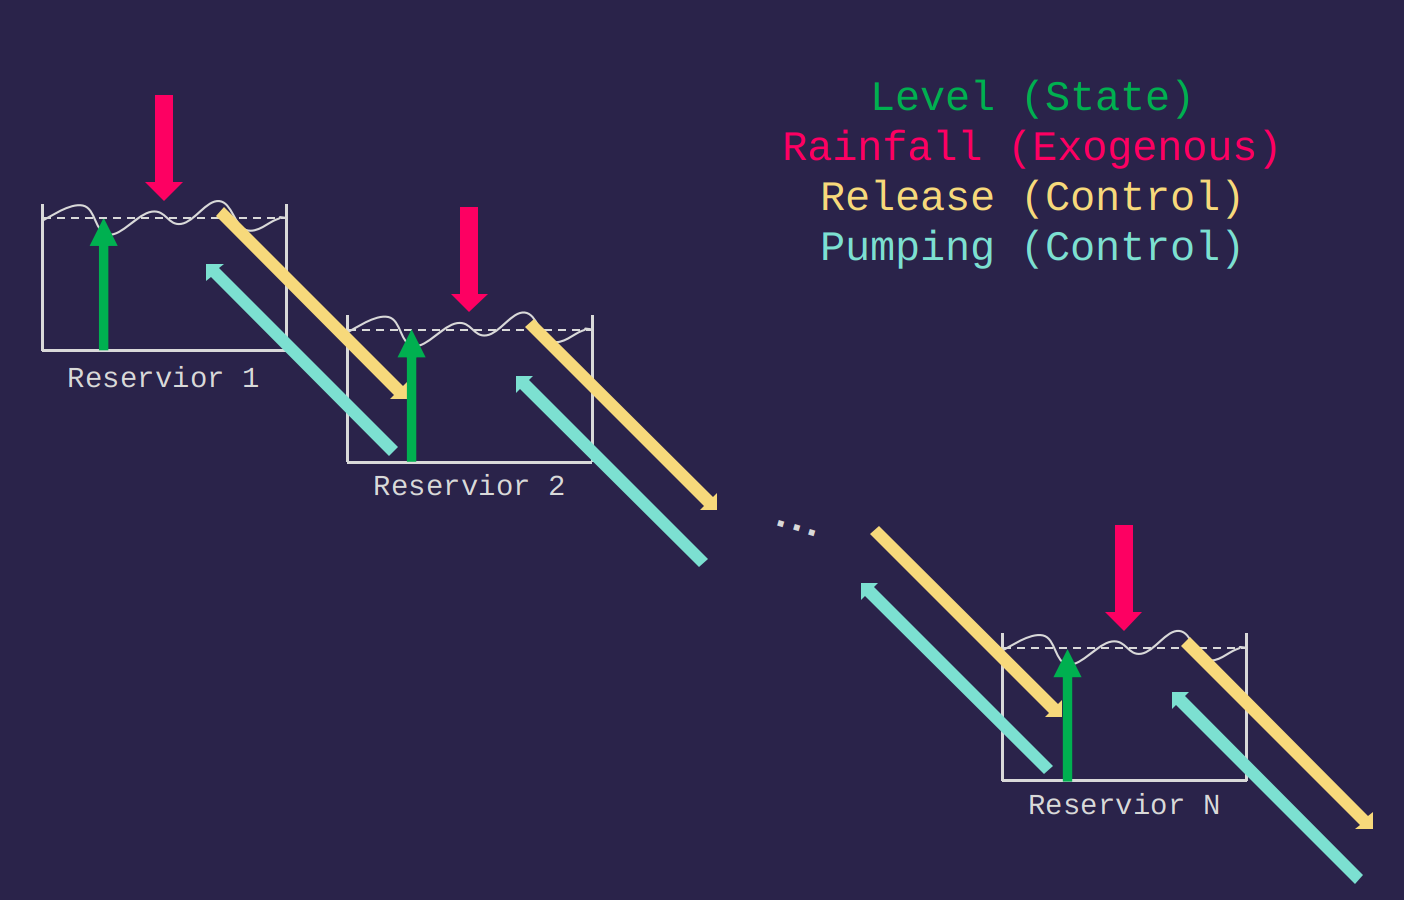
\includegraphics[width=\linewidth]{figs/Schematic.png}
	\caption{Schematic Description of the Problem}
	\label{fig:schematic}
\end{figure}

\section*{Description}

The \gls{chrp} is a classic example used in the teaching of optimal control and optimization as well as in evaluating the performance of solvers. By selecting the problem constraints the problem can be made simpler or more complex. In this document a maximalist formulation of the problem is presented with commentary and potential simplifications are noted. The purpose of this example is to show how to formulate various types of constraints and how to implement these in code. Deterministic and stochastic formulations are shown separately.

The \gls{chrp} concerns the optimal time-varying control of a series of $N$ interconnected reservoirs gated by hydroelectric dams over $M$ time-steps. The reservoirs are not necessarily of equal capacity. The dams are capable of generating electricity when water is released and capable of pumping water at the cost of expending electricity. Each of the generators and pumps is limited to function within given ranges of flow rates. Generation and pumping power are assumed to be proportional to flow-rate squared. Each generator and pump costs a given amount of energy to turn on and to turn off. All reservoirs are subject to rainfall and evaporation (represented as positive and negative flows). Each reservoir level must be maintained within a given range. After reservoir $N$ there is an assumed reservoir of infinite capacity. All reservoirs must be returned to their initial levels at the end of the period of optimization. All reservoirs are connected to the same electricity grid. The grid is also used to provide power for surrounding areas providing time-varying demand for electricity which the cascading reservoir hydroelectric system must meet or the system operator will have to pay transmission fees to buy the difference in power. Excess power produced may be sold via transmission. The objective of the operator is to maximize profits from the production of electricity by finding optimal time-varying controls for all generators and pumps.

\section*{Deterministic Formulation}

The objective of the problem is

\begin{gather}
	\min_{u\in U}\quad
	\sum_{r\in R}\sum_{t\in T}(u_{r,t}^{g})^2c_{r,t}^{g}+
	\sum_{r\in R}\sum_{t\in T}(u_{r,t}^{p})^2c_{r,t}^{p}+
	\sum_{t\in T}u_{t}^{t}c_{t}^{t}+\\
	\sum_{r\in R}\sum_{t\in T}\begin{cases}
		c_{r,t}^{gc} & \Delta(u_{r,t}^{gc})=1\\
		0 & \Delta(u_{r,t}^{gc})=0\\
		c_{r,t}^{gc} & \Delta(u_{r,t}^{gc})=-1
	\end{cases}+
	\sum_{r\in R}\sum_{t\in T}\begin{cases}
		c_{r,t}^{pc} & \Delta(u_{r,t}^{pc})=1\\
		0 & \Delta(u_{r,t}^{pc})=0\\
		c_{r,t}^{pc} & \Delta(u_{r,t}^{pc})=-1
	\end{cases}\label{eq:obj}
\end{gather}

where $U=[u^g,u^p,u^t,u^{gc},u^{pc}]$ is the vector of problem controls containing, in order, generator flow rate, pump flow rate, transmission power, generator unit commitment, and pump unit commitment, $R$ is the set of reservoirs, $T$ is the set of discrete time-steps of the problem, and $C=[c^g,c^p,c^t,c^{gc},c^{pc}]$ is a vector of constant cost multipliers for the problem controls. $\Delta$ indicates the function $\Delta(x_t)=x_t-x_{t-1}$.\\

The optimization is subject to the following constraints, beginning with those which are system wide. The first constraint is conservation of energy, it is formulated as

\begin{equation}
	\sum_{r\in R}\sum_{t\in T}(u_{r,t}^{g})^2+
	\sum_{r\in R}\sum_{t\in T}(u_{r,t}^{p})^2+
	\sum_{t\in T}u_{t}^{t}+
	\sum_{t\in T}y_{t}^{e}=0\label{eq:coe}
\end{equation}

where $y^e$ is the local time-varying power demand and is exogenous. the second constraint is conservation of mass, it is formulated as

\begin{equation}
	\sum_{r\in R}\sum_{t\in T}u_{r,t}^{g}+
	\sum_{r\in R}\sum_{t\in T}u_{r,t}^{p}+
	\sum_{r\in R}\sum_{t\in T}y_{r,t}^{f}=0\label{eq:com}
\end{equation}

where $y^f$ is the time-varying flow due to rainfall/evaporation at each reservoir.\\

Each reservoir has a range of operation in which its level must be maintained. The operating range lower bound constraint is formulated as

\begin{equation}
	\sum_{t\in T_K}^{L}[u_{r,t}^{g}+u_{r,t}^{p}+y_{r,t}^{f}]\geq LB_{r} : T_K=T_0,T_1,...,T_k \quad\forall k \in 0,1,...,M \quad\forall r \in R \label{eq:lb}
\end{equation}

where $LB$ is the lower boundary of the operating range. This constraint computes the state (reservoir) level for each time step by summing the in and outflows from that reservoir in all previous time-steps. This is a "factorial" constraint and it is easy to conceptualize in matrix form. It is equivalent to multiplying an $N$ by $N$ matrix with zeros above diagonal and ones on and below diagonal (called a Lower traingular matrix) by the vectors of in and out flows then summing. A version of this constraint is produced for each reservoir. In matrix form Equation \eqref{eq:lb} would take the form seen in Equation \eqref{eq;mat_lb}.

\begin{equation}
	\begin{bmatrix}
		1 & 0 & \dots & 0\\
		1 & 1 & \dots & 0\\
		\vdots & \vdots &\ddots & \\
		1 & 1 & & 1
	\end{bmatrix}
	\begin{bmatrix}
		u_{r,0}^g \\ u_{r,1}^g \\ \vdots \\ u_{r,N}^g
	\end{bmatrix}+
	\begin{bmatrix}
		1 & 0 & \dots & 0\\
		1 & 1 & \dots & 0\\
		\vdots & \vdots &\ddots & \\
		1 & 1 & & 1
	\end{bmatrix}
	\begin{bmatrix}
		u_{r,0}^p \\ u_{r,1}^p \\ \vdots \\ u_{r,N}^p
	\end{bmatrix}+
	\begin{bmatrix}
		y_{r,0}^f \\ y_{r,1}^f \\ \vdots \\ y_{r,N}^f
	\end{bmatrix}\geq UB_r \quad \forall r \in R
	\label{eq;mat_lb}
\end{equation}

The upper bound constraint is formulated similarly as

\begin{equation}
	\sum_{t\in T_K}^{L}[u_{r,t}^{g}+u_{r,t}^{p}+y_{r,t}^{f}]\leq UB_{r} : T_K=T_0,T_1,...,T_k \quad\forall k \in 0,1,...,M \quad\forall r \in R \label{eq:ub}
\end{equation}

where $UB$ is the upper boundary of the operating range. The final state value is enforced by the constraint

\begin{equation}
	\sum_{t\in T}^{L}[u_{r,t}^{g}+u_{r,t}^{p}+y_{r,t}^{f}]=FS_{r} \quad\forall r \in R \label{eq:fs}
\end{equation}

where $FS$ is the final state (level) value for each reservoir. The final constraint is unit commitment. The unit commitment constraint enforces the nonlinear operations of the generators and pumps using two linear variables (one continuous and one binary). The unit commitment constraints are posed as

\begin{gather}
	f_{r,t}^{g,min}u_{r,t}^{gc}-u_{r,t}^{g}\leq 0 \quad\forall r \in R \quad\forall t \in T\\
	f_{r,t}^{g,max}u_{r,t}^{gc}-u_{r,t}^{g}\geq 0 \quad\forall r \in R \quad\forall t \in T\\
	f_{r,t}^{p,min}u_{r,t}^{pc}-u_{r,t}^{p}\leq 0 \quad\forall r \in R \quad\forall t \in T\\
	f_{r,t}^{p,max}u_{r,t}^{pc}-u_{r,t}^{p}\geq 0 \quad\forall r \in R \quad\forall t \in T
\end{gather}

where $f^{g,min}$ and $f^{g,max}$ and the minimum and maximum operating flow rates for each generator and $f^{p,min}$ and $f^{p,max}$ and the minimum and maximum operating flow rates for each pump.

There are many possible simplifications to the 

\section*{Stochastic Formulation}

In the deterministic formulation of the problem the exogenous variables, rainfall and local electricity demand are know \textit{a priori}. This is not reflective of real-world operation. There will always be some uncertainty surrounding exogenous variables. In the \gls{schrp} it is assumed that the operator must pass a time-varying transmission schedule to the greater grid dispatch controller before the period of operation in question. The dispatch controller uses this information to optimize the greater grid's coordinated operation and thus, deviations from the agreed transmission schedule are discouraged. In this scenario, the agreed schedule is the baseline and deviations from the agreed schedule are subject to a fee. The job of the reservoir system operator is to provide a transmission schedule which will allow for highest expected profit across a range of scenarios which are not necessarily equally likely to occur.

There are two types of control variables in stochastic programming. Herein these will be called "general" and "specific" variables but they are also called first and second stage variables. General variables are those which apply in all scenarios and specific variables are those which apply in only one scenario. In this problem the transmission schedule is general and the generation, pumping, and transmission controls are all specific.

The objective of the \gls{schrp} is

\begin{gather}
	\min_{u\in U}\quad
	\sum_{s \in S}\sum_{r\in R}\sum_{t\in T}p_s(u_{s,r,t}^{g})^2c_{s,r,t}^{g}+
	\sum_{s \in S}\sum_{r\in R}\sum_{t\in T}p_s(u_{s,r,t}^{p})^2c_{s,r,t}^{p}+
	\sum_{s \in S}\sum_{t\in T}p_su_{s,t}^{t}c_{s,t}^{t}+\\
	\sum_{s \in S}\sum_{r\in R}\sum_{t\in T}p_s\begin{cases}
		c_{s,r,t}^{gc} & \Delta(u_{s,r,t}^{gc})=1\\
		0 & \Delta(u_{s,r,t}^{gc})=0\\
		c_{s,r,t}^{gc} & \Delta(u_{s,r,t}^{gc})=-1
	\end{cases}+
	\sum_{s \in S}\sum_{r\in R}\sum_{t\in T}p_s\begin{cases}
		c_{s,r,t}^{pc} & \Delta(u_{s,r,t}^{pc})=1\\
		0 & \Delta(u_{s,r,t}^{pc})=0\\
		c_{s,r,t}^{pc} & \Delta(u_{s,r,t}^{pc})=-1
	\end{cases}\label{eq:obj}
\end{gather}

where $S$ is the set of discrete scenarios considered and $p$ is the probability of each scenario meaning that the objective function is weighted by probability. It should be noted that all variables in the objective function are specific variables. Because the \textit{a priori} transmission schedule is used as a baseline and $u^t$ now represents deviation from this baseline, the transmission schedule is not an immediate determinant of profit. The transmission schedule will show up in the constraints.

The conservation of energy constraint is

\begin{equation}
	\sum_{s \in S}\sum_{r\in R}\sum_{t\in T}(u_{s,r,t}^{g})^2+
	\sum_{s \in S}\sum_{r\in R}\sum_{t\in T}(u_{s,r,t}^{p})^2+
	\sum_{s \in S}\sum_{t\in T}[u_{t}^{ts}+u_{s,t}^{t}]+
	\sum_{s \in S}\sum_{t\in T}y_{s,t}^{e}=0\label{eq:coe_s}
\end{equation}

where $u^{ts}$ is the transmission schedule for each time step. The remaining constraints are:

\begin{equation}
	\sum_{s \in S}\sum_{r\in R}\sum_{t\in T}u_{s,r,t}^{g}+
	\sum_{s \in S}\sum_{r\in R}\sum_{t\in T}u_{s,r,t}^{p}+
	\sum_{s \in S}\sum_{r\in R}\sum_{t\in T}y_{s,r,t}^{f}=0\label{eq:com_s}
\end{equation}

\begin{equation}
	\sum_{s \in S}\sum_{t\in T_K}^{L}[u_{s,r,t}^{g}+u_{r,t}^{p}+y_{s,r,t}^{f}]\geq LB_{s,r} : T_K=T_0,T_1,...,T_k \quad\forall k \in 0,1,...,M \quad\forall r \in R \quad\forall s \in S \label{eq:lb_s}
\end{equation}

\begin{equation}
	\sum_{s \in S}\sum_{t\in T_K}^{L}[u_{s,r,t}^{g}+u_{r,t}^{p}+y_{s,r,t}^{f}]\leq UB_{s,r} : T_K=T_0,T_1,...,T_k \quad\forall k \in 0,1,...,M \quad\forall r \in R \quad\forall s \in S \label{eq:ub_s}
\end{equation}

\begin{equation}
	\sum_{s \in S}\sum_{t\in T}^{L}[u_{s,r,t}^{g}+u_{s,r,t}^{p}+y_{s,r,t}^{f}]=FS_{s,r} \quad\forall r \in R \quad\forall s \in S \label{eq:fs_s}
\end{equation}

\begin{gather}
	f_{s,r,t}^{g,min}u_{s,r,t}^{gc}-u_{s,r,t}^{g}\leq 0 \quad\forall r \in R \quad\forall t \in T \quad\forall s \in S\\
	f_{s,r,t}^{g,max}u_{s,r,t}^{gc}-u_{s,r,t}^{g}\geq 0 \quad\forall r \in R \quad\forall t \in T \quad\forall s \in S\\
	f_{s,r,t}^{p,min}u_{s,r,t}^{pc}-u_{s,r,t}^{p}\leq 0 \quad\forall r \in R \quad\forall t \in T \quad\forall s \in S\\
	f_{s,r,t}^{p,max}u_{s,r,t}^{pc}-u_{s,r,t}^{p}\geq 0 \quad\forall r \in R \quad\forall t \in T \quad\forall s \in S
\end{gather}


\end{document}